
\lstset{
     literate=%
         {á}{{\'a}}1
         {í}{{\'i}}1
         {é}{{\'e}}1
         {ý}{{\'y}}1
         {ú}{{\'u}}1
         {ó}{{\'o}}1
         {ě}{{\v{e}}}1
         {š}{{\v{s}}}1
         {č}{{\v{c}}}1
         {ř}{{\v{r}}}1
         {ž}{{\v{z}}}1
         {ď}{{\v{d}}}1
         {ť}{{\v{t}}}1
         {ň}{{\v{n}}}1                
         {ů}{{\r{u}}}1
         {Á}{{\'A}}1
         {Í}{{\'I}}1
         {É}{{\'E}}1
         {Ý}{{\'Y}}1
         {Ú}{{\'U}}1
         {Ó}{{\'O}}1
         {Ě}{{\v{E}}}1
         {Š}{{\v{S}}}1
         {Č}{{\v{C}}}1
         {Ř}{{\v{R}}}1
         {Ž}{{\v{Z}}}1
         {Ď}{{\v{D}}}1
         {Ť}{{\v{T}}}1
         {Ň}{{\v{N}}}1                
         {Ů}{{\r{U}}}1    
}

\chapter{Úvod}
úvod

\chapter{Parametrické 3d modely}
Hlavná výhoda parametrických modelov voči priamemu  s



\chapter{Geometrické tvary}
\label{chapt:Geometrické_tvary}
štruktúra objektov



\chapter{Geometrické operácie}
Geometrické operácie sa delia na 4 typy podľa toho, aký typ objektu sa dá pomocou nich vytvoriť. Sú to operácie bodové, úsečkové, plošné a priestorové. Na vytváranie zložitejších objektov je potrebné využívať jednoduchšie geometrické objekty. 

Všetky geometrické operácie sa dajú zapisovať pomocou textovej podoby. Tento textový zápis operácii je taktiež uvedený pri jednotlivých operáciach nižšie. 
Textová podoba geometrickej operácie sa začína názvom použitej geometrickej operácie nasledovaný parametrami uvedenými v zátvorkách \( a \), oddelenými znakom ','.  U jednotlivých parametrov sa počiatočné a koncové whitespace znaky ignorujú.
Pri parametroch tymu $Float$ je možné vytvoriť názov, podľa ktorého sa bude dať na daný parameter neskôr pristupovať. 
Tento názov sa zadáva po parametre 
Parametre jednotlivých geometrických operácii sú zadané nižšie. 
Jednotlivé operácie sa oddelujú bodkočiarkou ';'. 
Táto textová podoba geometrických operácii sa používa aj pre uloženie do súboru a jeho neskoršie načítanie. 

Ako príklad uvádzam vytvorenie ihlana s kruhovou podstavou s polomerom 5 a výškou 10:
\begin{itemize}
    \item Na vytvorenie ihlana je potrebné najprv vytvoriť bod na pozícii XYZ, napr. $\left [ 1, 2, 3 \right ]$, ktorý bude slúžiť ako stred kruhovej podstavy.
	\begin{lstlisting}
	Point(bod podstavy, 1, 2, 3 ,0);
	\end{lstlisting}
	\item Na vytvorenie kruhu (podstavy ihlana) je potrebný polomer a normála. Ako normálu je možné využiť smer ľubovolnej úsečky, ale keďže zatiaľ žiadnu úsečku vytvorenú nemáme, je potrebné ju vytvoriť. Úsečka sa skladá z dvoch bodov a to počiatočného a koncového. Ako normála sa použije normalizovaný vektor medzi bodom počiatočným a koncovým \ref{eq:normalizacia_usecky}.

	\begin{equation}
		\overrightarrow{normal\_vector}=
		\frac{end\_point - begin\_point}{
		\left \|  end\_point - begin\_point \right \|}
	\label{eq:normalizacia_usecky}
	\end{equation}

	\begin{lstlisting}
	Point(počiatočný bod, 0, 0, 0, 0);
	Point(koncový bod, 1, 1, 1, 0);
	Line(normála, počiatočný bod, koncový bod, 0);
	\end{lstlisting}
	\item Keď už je normála vytvorená, je možné vytvoriť kruh s polomerom 5.
	\begin{lstlisting}
	Circle(podstava, bod podstavy, 5, normála, 0) 
	\end{lstlisting}
	\item Ostáva vytvoriť samotný ihlan s výškou 10.
	\begin{lstlisting}
	Pyramid(ihlan s kruhovou podstavou, podstava, 10, 1)
	\end{lstlisting}
\end{itemize}

\todo{ako vyzerá tento sled operácii pomocou graphviz a v 3D}

Ďalej nasleduje výpis podporovaných geometrických operácii, kde pri každej operácii sa nachádza jednoduchý popis, formát zápisu tejto operácie a grafové zobrazenie vytvorenia tejto operácie.


\section{Bodové operácie}
Bodové operácie sú operácie, ktorých výstupom je bod.
\subsection{Bod}
Základná stavebná jednotka každého objektu. Na vytvorenie bodu je potrebné zadať jeho pozíciu v osiach X, Y a Z. Bod môže byť zadaný buď v absolútnej alebo v relatívnej pozícii, kedy je jeho pozícia závislá na polohe iného bodu.
\begin{lstlisting}
    Point(string name, float X, float Y, float Z,float visibility) 
    Point(string name, float X, float Y, float Z,Point Parent,
        float visibility)
\end{lstlisting}
\begin{figure}[H]
	\centering
	
\includegraphics[width=0.5\textwidth]{obrazky-figures/placeholder.pdf}
	\caption{text}
	\label{fig:1}
\end{figure}

\subsection{Lineárna interpolácia}
Výsledná pozícia bodu závisí od zadanej vzdialenosti od počiatočného bodu. Táto vzdialenosť môže byť zadaná dĺžkou alebo percentuálne, kde 50% vytvorí bod uprostred počiatočného a koncového bodu. 
Keďže percentá sa zadávajú tiež vo formáte desatinného čísla ($Float$), bolo potrebné tieto operácie rozlíšiť. Pre zadanie vzdialenosti podľa dĺžky, sa zadáva operácia \texttt{LinearInterpolationDist}, 
pre percentuálnu vzdialenosť je operácia \texttt{LinearInterpolationPerc}.
\begin{lstlisting}
    LinearInterpolationDist(string name, Point fromPoint,Point toPoint,
        float distance,float visibility)
    LinearInterpolationPerc(string name, Point fromPoint,Point toPoint,
        float percentage,float visibility)
\end{lstlisting}

\begin{figure}[H]
	\centering
	
\includegraphics[width=0.4\textwidth]{obrazky-figures/placeholder.pdf}
	
\includegraphics[width=0.4\textwidth]{obrazky-figures/placeholder.pdf}
	\caption{text}
	\label{fig:1}
\end{figure}


\begin{equation}
\begin{split}
    Vector3 normal = (p2.Position - p1.Position).Normalize();
    \\
	Point ReturnPoint = p1 + normal * distance;
	\label{eq:LiearnInterpolationDist}
\end{split}
\end{equation}
\begin{equation}
    Point ReturnPoint = p1 + percentage * (p2 - p1);
    \textbf{N} \cdot (\textbf{P} - \textbf{P3}) = 0
	\label{eq:LiearnInterpolationPerc}
\end{equation}


\subsection{Priesečník plochy a úsečky}
http://paulbourke.net/geometry/pointlineplane/

Pri tejto operácii sa používa ľubovolný plošný objekt ako rovina a úsečka ako priamka. Táto geometrická operácia vytvorí bod v mieste, kde sa priamka pretína s rovinou. 
\begin{figure}[H]
	\centering
	
\includegraphics[width=0.5\textwidth]{obrazky-figures/placeholder.pdf}
	\caption{text}
	\label{fig:GraphIntersection_Plane_Line}
\end{figure}


Rovnica pre rovinu, ktorá je tvorená bodom \texttt{P\textsubscript{3}} nachádzajúcom sa na rovine a normálou N, je \ref{eq:rovnicaPlochy_intersection}. 
\begin{equation}
    \textbf{N} \cdot (\textbf{P} - \textbf{P3}) = 0
	\label{eq:rovnicaPlochy_intersection}
\end{equation}

Rovnica pre priamku, ktorá je určená bodmi \texttt{P\textsubscript{1}} a \texttt{P\textsubscript{2}}
\ref{eq:rovnicaPriamky_intersection}
\begin{equation}
	\textup{P}=\textbf{P1}+u (\textbf{P2}-\textbf{P1})
    \label{eq:rovnicaPriamky_intersection}
\end{equation}
	
Bod \texttt{P} označuje priesečník medzi rovinou a priamkou. Pomocou substitúcie získame rovnicu \ref{eq:rovnicaPriesecniku}.

\begin{equation}
	\textbf{N} \cdot (\textbf{P1}+u(\textbf{P2}-\textbf{P1}))) = \textbf{N} \cdot \textbf{P3}
    \label{eq:rovnicaPriesecniku}
\end{equation}

Po vyriešení tejto rovnice dostaneme rovnicu \ref{eq:rovnicaPriesecnikuSolved}. Výslednú pozíciu bodu dostaneme dosadením $u$ do rovnice pre  priamku \ref{eq:rovnicaPriamky_intersection}.
\begin{equation}
	u=\frac
{\textbf{N} \cdot (\textbf{P3}-\textbf{P1})}
{\textbf{N} \cdot (\textbf{P2}-\textbf{P1})}
    \label{eq:rovnicaPriesecnikuSolved}
\end{equation}

\begin{figure}[H]
	\centering
	
\includegraphics[width=0.5\textwidth]{obrazky-figures/placeholder.pdf}
	\caption{text}
	\label{fig:1}
\end{figure}



\begin{lstlisting}
	Intersection\_Plane\_Line(string name, Line lineName, Sufrace surfaceName, bool visible = true)
	//	Alternative:
	//	Intersection(string name, Line lineName, Sufrace surfaceName)
	//	Example:
	//		Intersection\_Plane\_Line(PointName,  lineName, surfaceName) //- Create Point on position where Line with name "lineName" intersecting Surface with name "surfaceName"

\end{lstlisting}

\subsection{SurfaceMiddle}


\begin{lstlisting}
	SurfaceMiddle(string name, Surface surfaceName, bool visible = true) //Create point on position of middle of entered surface
	//	Example:
	//		SurfaceMiddle(PointName, Circle)	//- Create Point on center of Circle
	//		SurfaceMiddle(PointName, Rectangle)	//- Create Point on middle of Rectangle
	//		SurfaceCenter(PointName, Shape)		//- Create Point on middle of shape 
	//		SurfaceMiddle(PointName, Shape)		//- Create Point on middle of shape - centroid (sum of points / count of points)
\end{lstlisting}

\begin{figure}[H]
	\centering
	
\includegraphics[width=0.5\textwidth]{obrazky-figures/placeholder.pdf}
	\caption{text}
	\label{fig:1}
\end{figure}

\subsection{Stred objektu}
https://www.gamedev.net/forums/topic/468405-center-of-a-3d-object/

Existuje množstvo možností ako získať stred 3D objektu. Do tejto práce som implementoval 2 z nich. 
\subsubsection{Stred ohraničujúceho kvádra}
Prejde všetky body a zoberie maximálnu a minimálnu hodnotu v osiach X, Y a Z. Takto dostaneme ohraničujúci kváder (Bounding box) a ako výsledný bod sa zoberie stred tohoto kvádra.

		ObjectMiddle,//(string name, Object3D ObjectName, bool visible = true) //Create point on position of middle of entered object
		
\begin{figure}[H]
	\centering
	
\includegraphics[width=0.5\textwidth]{obrazky-figures/placeholder.pdf}
	\caption{text}
	\label{fig:1}
\end{figure}

\subsubsection{Priemerný stred všetkých bodov} 
Pri tejto operácii sa spočítajú koordináty všetkých bodov. To vytvorí tri veľké čísla, ktoré sa následne vydelia počtom bodov.
		ObjectCenter,//(string name, Object3D ObjectName, bool visible = true) //Create point on position of center of entered object

\begin{figure}[H]
	\centering
	
\includegraphics[width=0.5\textwidth]{obrazky-figures/placeholder.pdf}
	\caption{text}
	\label{fig:1}
\end{figure}

\subsection{Začiatok a koniec úsečky}
Aby sa dalo pristupovať k začiatočnému a koncovému bodu úsečky, vytvoril som operácie \texttt{LineFirstPoint} a \textt{LineSecondPoint}.
\label{sec:begandendofline}

\begin{lstlisting}
    LineFirstPoint(string name, Line lineName, bool visible = true)
	LineSecondPoint(string name, Line lineName, bool visible = true)
	\label{eq:LINEBegAndEnd}
\end{lstlisting}
		
		


\begin{figure}[H]
	\centering
	
\includegraphics[width=0.5\textwidth]{obrazky-figures/placeholder.pdf}
	\caption{text}
	\label{fig:1}
\end{figure}



	






\section{Úsečkové operácie}


\subsection{Úsečka}
Úsečka sa nachádza v mnohých operáciach ako parameter, kde zastupuje úlohu smerového vektoru. Každá úsečka s začína počiatočným bodo a končí koncvým bodom. Pre získanie počiatočného a koncového bodu je operácia \ref{sec:begandendofline}.

		Line(string lineName, Point p1, Point p2, bool visible = true) //create line, where p1 is start point and p2 is end point

\begin{figure}[H]
	\centering
	
\includegraphics[width=0.5\textwidth]{obrazky-figures/placeholder.pdf}
	\caption{text}
	\label{fig:1}
\end{figure}

\subsection{Normalizovanie veľkosti úsečky}
		LineNormalize,//(string lineName, Line l, bool visible = true)

\begin{figure}[H]
	\centering
	
\includegraphics[width=0.5\textwidth]{obrazky-figures/placeholder.pdf}
	\caption{text}
	\label{fig:1}
\end{figure}

\subsection{Zmena dĺžky úsečky}
		LineChangeLengthDist,//(string lineName, Line l, float distance, bool visible = true)
		LineChangeLengthPerc,//(string lineName, Line l, float percent, bool visible = true) //percent = (0;1>

\begin{figure}[H]
	\centering
	
\includegraphics[width=0.5\textwidth]{obrazky-figures/placeholder.pdf}
	\caption{text}
	\label{fig:1}
\end{figure}


\subsection{Lineárna interpolácia}

		// these commands are based on page http://paulbourke.net/geometry/pointlineplane/
		MinLineBetweenLineAndLine,//(string lineName, Line l1, Line l2, bool visible = true)

\begin{figure}[H]
	\centering
	
\includegraphics[width=0.5\textwidth]{obrazky-figures/placeholder.pdf}
	\caption{text}
	\label{fig:1}
\end{figure}

\subsection{Lineárna interpolácia}
		MinLineBetweenPointAndLine,//(string lineName, Point p, Line l, bool visible = true)

\begin{figure}[H]
	\centering
	
\includegraphics[width=0.5\textwidth]{obrazky-figures/placeholder.pdf}
	\caption{text}
	\label{fig:1}
\end{figure}

\subsection{Lineárna interpolácia}
		MinLineBetweenPointAndSurface,//(string lineName, Point p, Surface s, bool visible = true)

\begin{figure}[H]
	\centering
	
\includegraphics[width=0.5\textwidth]{obrazky-figures/placeholder.pdf}
	\caption{text}
	\label{fig:1}
\end{figure}


\subsection{Lineárna interpolácia}
		///Alternative:
		MinLine,//(string lineName, Object o1, Object o2, bool visible = true) //Supported are only : [Line,Line], [Point,Line], [Point, Surface]


\begin{figure}[H]
	\centering
	
\includegraphics[width=0.5\textwidth]{obrazky-figures/placeholder.pdf}
	\caption{text}
	\label{fig:1}
\end{figure}



\subsection{Lineárna interpolácia}
		SurfaceNormal,//(string lineName, Surface s, bool visible = true) // return normal vector of surface


\begin{figure}[H]
	\centering
	
\includegraphics[width=0.5\textwidth]{obrazky-figures/placeholder.pdf}
	\caption{text}
	\label{fig:1}
\end{figure}



\subsection{Lineárna interpolácia}
		LineRelocationByPoint,//(string lineName, Line l, Point p, bool visible = true)


\begin{figure}[H]
	\centering
	
\includegraphics[width=0.5\textwidth]{obrazky-figures/placeholder.pdf}
	\caption{text}
	\label{fig:1}
\end{figure}

\subsection{Lineárna interpolácia}
		//OrthogonalLeastSquares,//(string lineName, Point p1, Point p2, Point p3, ..., bool visible = true) //min 3

\begin{figure}[H]
	\centering
	
\includegraphics[width=0.5\textwidth]{obrazky-figures/placeholder.pdf}
	\caption{text}
	\label{fig:1}
\end{figure}


\subsection{Lineárna interpolácia}
		//CrossProductLP,//(string lineName, Line l, Point p, bool visible = true)
		CrossProduct,//(string lineName, Line l1, Line l2, bool visible = true)

\begin{figure}[H]
	\centering
	
\includegraphics[width=0.5\textwidth]{obrazky-figures/placeholder.pdf}
	\caption{text}
	\label{fig:1}
\end{figure}





\section{Plošné operácie}


\subsection{Lineárna interpolácia}
	AddWidthToLine,//(string surfaceName, Line l, float width, Point surfacePoint, short type, bool visible = true)
	//AddWidthToLine(string surfaceName, Line l, float width, Vector3 normalVector, short type, bool visible = true)
//create Rectangle from Line l
/*type:
	0 - width/2 to left, width/2 to right
	1 - width to left
	2 - width to right
	*/
	//if normal vector is not perpendicular to line, as normal is used normalized dot product between line and normal vector
	//if normal vector is same direction as line normal, exception occure
	//If surface point is not on line l, exception occure

\begin{figure}[H]
	\centering
	
\includegraphics[width=0.5\textwidth]{obrazky-figures/placeholder.pdf}
	\caption{text}
	\label{fig:1}
\end{figure}

\subsection{Lineárna interpolácia}
	Circle,//(string surfaceName, Point center, float radius, Line lineNormal, bool visible = true)
	//Circle(string surfaceName, Point center, Point outlinePoint, Point planePoint, bool visible = true)

\begin{figure}[H]
	\centering
	
\includegraphics[width=0.5\textwidth]{obrazky-figures/placeholder.pdf}
	\caption{text}
	\label{fig:1}
\end{figure}


\subsection{Lineárna interpolácia}
	Triangle,//(string surfaceName, Line l, Point p, bool visible = true)
	//Triangle(string surfaceName, Point p1, Point p2, Point p3, bool visible = true)

\begin{figure}[H]
	\centering
	
\includegraphics[width=0.5\textwidth]{obrazky-figures/placeholder.pdf}
	\caption{text}
	\label{fig:1}
\end{figure}


\subsection{Lineárna interpolácia}
	//rectangle
	Rectangle,//(string surfaceName, Point center, float X, float Y, float Roll/*[0,360]*/, Line normal, bool visible = true)

\begin{figure}[H]
	\centering
	
\includegraphics[width=0.5\textwidth]{obrazky-figures/placeholder.pdf}
	\caption{text}
	\label{fig:1}
\end{figure}


\subsection{Lineárna interpolácia}
	Shape,//(string surfaceName, Point p1, Point p2, Point p3, ..., bool visible = true)//minimum 3 points 

\begin{figure}[H]
	\centering
	
\includegraphics[width=0.5\textwidth]{obrazky-figures/placeholder.pdf}
	\caption{text}
	\label{fig:1}
\end{figure}



\subsection{Lineárna interpolácia}
	Circumscribed,//(string surfaceName, Triangle t, bool visible = true) //Create circle over triangle

\begin{figure}[H]
	\centering
	
\includegraphics[width=0.5\textwidth]{obrazky-figures/placeholder.pdf}
	\caption{text}
	\label{fig:1}
\end{figure}

\subsection{Lineárna interpolácia}
	Inscribed,//(string surfaceName, Triangle t, bool visible = true)		//Create circle in triangle

\begin{figure}[H]
	\centering
	
\includegraphics[width=0.5\textwidth]{obrazky-figures/placeholder.pdf}
	\caption{text}
	\label{fig:1}
\end{figure}







\section{Priestorové operácie}


\subsection{Lineárna interpolácia}
Pyramid,//(string objectName, Surface s, float distance, bool visible = true) //Create Pyramid by distance from center
//Pyramid(string objectName, Surface s, Point p, bool visible = true) //Create Pyramid by Point

\begin{figure}[H]
	\centering
	
\includegraphics[width=0.5\textwidth]{obrazky-figures/placeholder.pdf}
	\caption{text}
	\label{fig:1}
\end{figure}


\subsection{Lineárna interpolácia}
To3D,//(string objectName, Surface s, float distance, bool visible = true) //add width to 

\begin{figure}[H]
	\centering
	
\includegraphics[width=0.5\textwidth]{obrazky-figures/placeholder.pdf}
	\caption{text}
	\label{fig:1}
\end{figure}


\subsection{Lineárna interpolácia}
SpericalCurvedSurface,//(string objectName, Surface s, float distance, bool visible = true)

\begin{figure}[H]
	\centering
	
\includegraphics[width=0.5\textwidth]{obrazky-figures/placeholder.pdf}
	\caption{text}
	\label{fig:1}
\end{figure}



\subsection{Lineárna interpolácia}
Cylinder,//(string objectName, Line l, float radius, bool visible = true)

\begin{figure}[H]
	\centering
	
\includegraphics[width=0.5\textwidth]{obrazky-figures/placeholder.pdf}
	\caption{text}
	\label{fig:1}
\end{figure}




\chapter{Grafické rozhranie}
Okrem programátorského rozhrania, som vytvoril aj jednoduché grafické užívateľské rozhranie pomocou knižnice QT. Toto grafické rozhranie umožňuje užívateľovi jednoduchšie správu tvorby geometrických objektov a to aj vďaka prehľadnému zoznamu použitých geometrických operácii a zoznamu referencovaných premenných. 

\section{Zoznam geometrických operácii}
Aby bolo jednoduchšie vytvárať objekty, grafické rozhranie umožňuje geometrické operácie pridať, upraviť, mazať a aj vložiť na ľubovoľné miesto. Tieto operácie je tiež možné ľubovolne presúvať. Keďže parametre operácii môžu odkazovať iba na predchádzajúce objekty, je nutné pri upravovaní, presúvaní a mazaní tieto parametre kontrolovať. Grafické rozhranie následne zobrazí, u ktorých operácii sa nachádzajú nevyhovujúce parametre a tieto objekty (a objekty na nich závislé) sa nebudú vykresľovať.

\todo{Zobrazenie grafického rozhrania}


\subsection{Pridanie, vloženie a úprava geometrických operácii} 
Dialógové okno umožňuje výber operácie,  ktorá sa má použiť, zo zoznamu geometrických operácii. V zozname sa nachádza názov geometrickej operácie, parametre ktoré operácia potrebuje a nápoveda, ktorá informuje užívateľa čo daná operácia robí.
Po vybraní operácie zo zoznamu, sa zobrazia v pravej časti dialógového okna parametre vybranej operácie. Ak je dialógové okno v režime úpravy (okno sa zobrazilo po dvojkliku na zozname geometrických operácii), sú pri vybraní rovnakého typu operácie tieto parametre už predvyplnené hodnotami zvolenej operácie na úpravu.

Ako prvý parameter je názov takto vytvoreného objektu, ktorý je pri novo vytváraných objektoch (režim okna pridanie alebo vloženie) predvyplnený, ale je možné ho upraviť na ľubovolnú hodnotu.  
Po názve objektu nasleduje viditeľnosť objektu, ktorá určuje, ako bude takto vytvorený objekt viditeľný. Pri hodnote viditeľnosti na $<=0$ je objekt neviditeľný a pri hodnote $>=1$ je objekt plne viditeľný. Ak je táto hodnota v rozmedzí (0-1) je tento objekt priehľadný. 
Ďalej nasledujú samotné parametre operácie typu $Float,  Point, Line, Surface$ a ďalšie. Parametrom typu $Float$ sa dá nastaviť názov, podľa ktorého sa na ne bude odkazovať. Tento názov ale nieje povinný a pre nereferencované parametre stačí nechať políčko prázdne. Parametre typu $Float$, ktoré sú týmto názvom pomenované, sa následne zobrazia aj v zozname referencovaných parametrov.
V poslednom stĺpci sa nachádza nápoveda k danému parametru.

Po zadaní hodnoty sa overuje, či je táto hodnota valídna pre daný parameter. To zahŕňa testovanie, či hodnota zadaná parametru $Float$ je desatinné číslo a pri ostatných parametroch sa testuje, či existuje objekt s rovnakým názvom ako bol zadaný a či je tento objekt správnym typom prípadne podtypom (viac o typoch objektov v kapitole  \ref{chapt:Geometrické_tvary}). Tiež sa testuje aj názov objektu a názov referencovaného parametra na unikátnosť.
Ak hodnota parametra nesplňuje niektorú požiadavku, je toto políčko označené červenou farbou pozadia, čo upozorňuje užívateľa na chybu. Ak je hodnota valídna, políčko sa označí zeleným pozadím. Prázdne políčko je označené bielim pozadím. 

\begin{figure}[hbt]
	\centering
	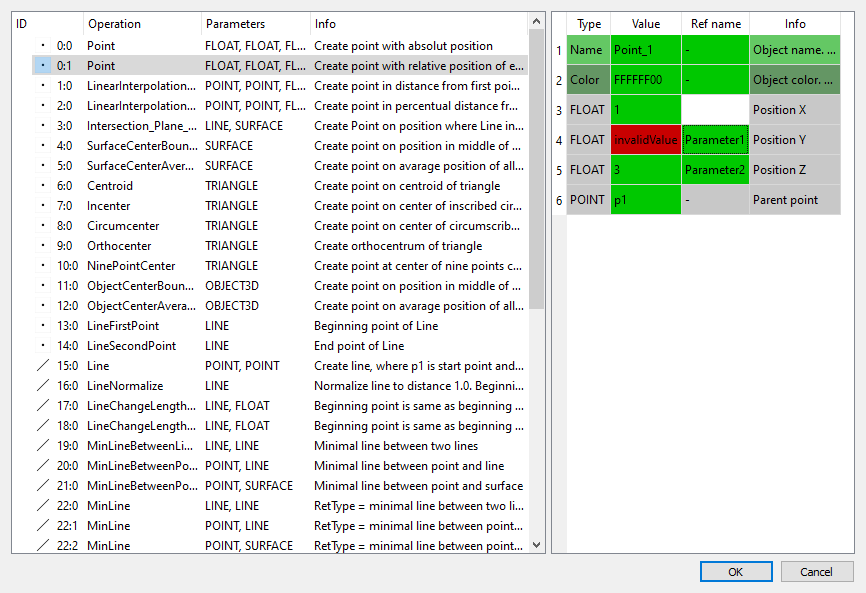
\includegraphics[width=1\textwidth]{obrazky-figures/Dialog.png}
	\caption{Dialógové okno na pridanie, vloženie a úpravu operácii}
	\label{fig:dialogWindow}
\end{figure}

\chapter{Ostáva spracovať}



\section{použitie niektorého parametru z už vytvorených geometrických objektov.}

\todo{príklad}

\section{Pridanie vykreslovania orientovaného grafu pomocou knižnice GraphViz}

\todo{ukážka kde sa má tento graf vykresliť a ako bude vyzerat}


